\documentclass[11pt,a4paper]{article}

\usepackage[utf8]{inputenc}
\usepackage[T1]{fontenc}
\usepackage[polish]{babel}
\usepackage{lmodern}
\usepackage[margin=2.5cm]{geometry}
\usepackage{amsmath}
\usepackage{graphicx}
\usepackage{booktabs}
\usepackage{float}
\usepackage{hyperref}

\graphicspath{{figures/}}

\title{Regresja logistyczna uczona spadkiem gradientu\\
\large Sieci neuronowe, lista 2: zbieżność a parametry uczenia}
\author{Jeremiasz Lizak}
\date{\today}

\begin{document}
\maketitle

\section{Cel}

Celem było zaimplementowanie regresji logistycznej od podstaw (NumPy, bez gotowych
optymalizatorów) i sprawdzenie, jak na zbieżność uczenia wpływają współczynnik uczenia,
sposób inicjalizacji wag i warunek stopu. Na koniec trzeba odpowiedzieć na pytanie, czy zła
parametryzacja uniemożliwia zbieżność, czy tylko ją wydłuża.

\section{Dane}

Wykorzystano zbiór UCI Heart Disease, czyli połączone pliki \texttt{processed.*.data} z czterech
ośrodków (Cleveland, Węgry, Szwajcaria, VA Long Beach). Po usunięciu duplikatów zostało
918 pacjentów i 13 cech. Zmienną \texttt{num} (0--4) zbinaryzowano: 0 oznacza brak choroby,
1--4 jej obecność. Klasa pozytywna stanowi 55\%.

Wartości zerowe w \texttt{trestbps} i \texttt{chol} potraktowano jako braki (dotyczy to głównie
danych ze Szwajcarii, gdzie cholesterolu nie mierzono). Dane podzielono warstwowo na zbiór
treningowy, walidacyjny i testowy w proporcji 60/20/20 (550/184/184). Imputacja, kodowanie
one-hot i standaryzacja są dopasowywane wyłącznie na zbiorze treningowym. Po przetworzeniu
model dostaje 27 cech.

Krzywe uczenia i wybór parametrów opierają się na zbiorze walidacyjnym. Zbiór testowy użyto
tylko raz, dla końcowej konfiguracji.

\section{Model i uczenie}

Model zwraca $p = \sigma(w^\top x + b)$, gdzie $\sigma(z) = 1/(1+e^{-z})$. Funkcją kosztu jest
średnia entropia krzyżowa (ujemna log-wiarygodność rozkładu Bernoulliego):
\[
  L(w,b) = -\frac{1}{n}\sum_{i=1}^{n}\bigl[y_i \log p_i + (1-y_i)\log(1-p_i)\bigr].
\]
Ponieważ $\partial L/\partial w = -\frac{1}{n}X^\top(y-p)$, krok spadku gradientu ma postać
\[
  w \leftarrow w + \eta\,\frac{1}{n}X^\top(y-p), \qquad
  b \leftarrow b + \eta\,\frac{1}{n}\sum_i (y_i-p_i).
\]
Uczenie jest pełnowsadowe (cały zbiór treningowy w każdej epoce). Pętla kończy się po
\texttt{n\_epochs} epokach albo wcześniej, gdy spadek kosztu między kolejnymi epokami jest
mniejszy niż \texttt{tol}.

Konfiguracja bazowa: $\eta = 0{,}1$, 5000 epok, $\texttt{tol} = 10^{-6}$, wagi z
$\mathcal{N}(0,\,0{,}01^2)$, $b = 0$. W każdym badaniu zmieniano jeden parametr, a każdy wariant
zapisano jako osobny run w MLflow. Jako punkt odniesienia policzono minimum kosztu
\texttt{LogisticRegression(penalty=None)} ze sklearn na tych samych danych:
$L^\ast = 0{,}3828$.

\section{Wyniki}

\subsection{Współczynnik uczenia}

\begin{table}[H]
\centering
\begin{tabular}{rccc}
\toprule
$\eta$ & koszt po 5000 epokach & epoki do $L \le 0{,}385$ & val F1 \\
\midrule
0,001 & 0,4536 & $> 20\,000$ & 0,860 \\
0,01  & 0,3896 & 9479  & 0,850 \\
0,1   & 0,3829 & 948   & 0,838 \\
1     & 0,3828 & 94    & 0,838 \\
10    & oscyluje 0,65--0,90 & nigdy & 0,783 \\
\bottomrule
\end{tabular}
\caption{Wpływ współczynnika uczenia (bez \texttt{tol}). Liczby epok do progu pochodzą
z dodatkowego uruchomienia z limitem 20\,000 epok.}
\end{table}

\begin{figure}[H]
\centering
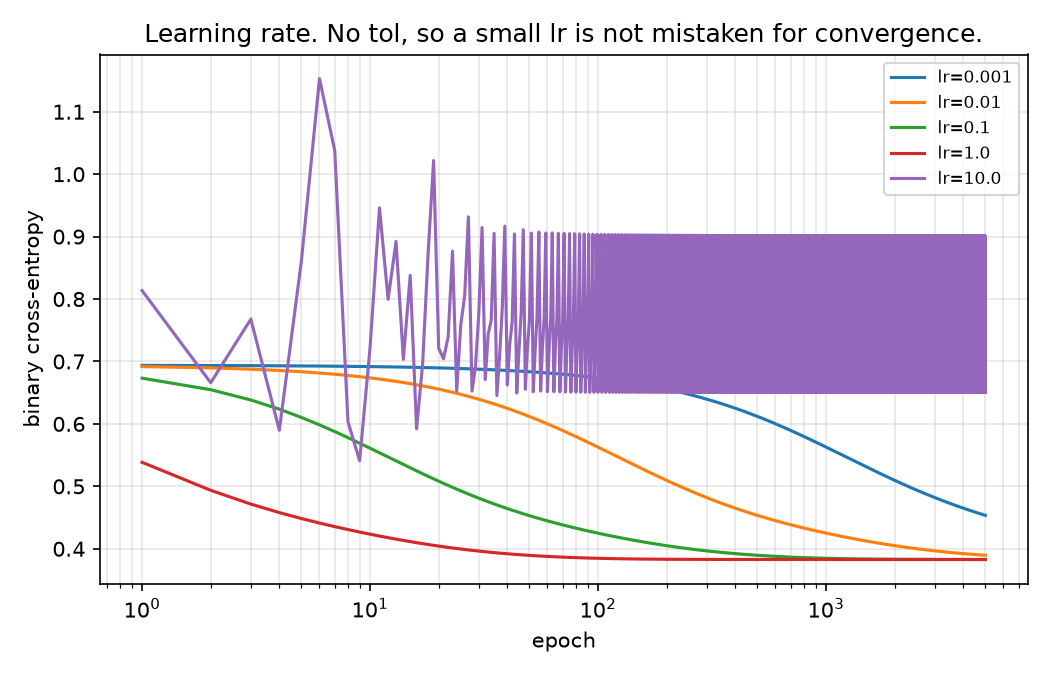
\includegraphics[width=0.8\textwidth]{lr.png}
\caption{Koszt treningowy dla różnych $\eta$ (oś epok logarytmiczna).}
\label{fig:lr}
\end{figure}

Dla $\eta$ od 0,001 do 1 koszt dąży do tego samego minimum. Zwiększenie $\eta$ dziesięciokrotnie
skraca uczenie mniej więcej dziesięciokrotnie (9479, 948, 94 epoki). Przy $\eta = 0{,}001$ limit
5000 epok to za mało i model kończy wyraźnie niedouczony.

Przy $\eta = 10$ koszt nie spada, tylko oscyluje (rys.~\ref{fig:lr}). Można to wyjaśnić
teoretycznie. Hesjan kosztu jest ograniczony przez $\frac{1}{4n}\tilde X^\top \tilde X$ (bo
$\sigma'(z) \le 1/4$), a $\tilde X$ to macierz cech z kolumną jedynek. Dla tych danych największa
wartość własna tej macierzy wynosi $\lambda \approx 0{,}87$. Spadek gradientu ma więc
gwarancję zbieżności dla $\eta < 2/\lambda \approx 2{,}3$, czyli $\eta = 1$ mieści się w tym
zakresie, a $\eta = 10$ nie.

\subsection{Inicjalizacja}

\begin{figure}[H]
\centering
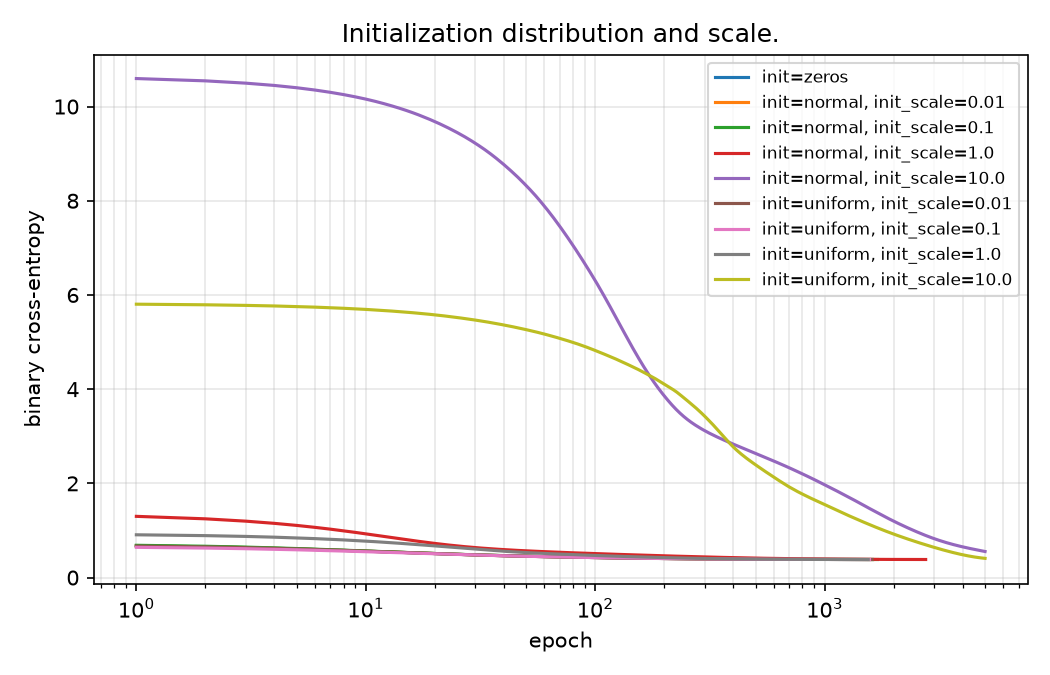
\includegraphics[width=0.8\textwidth]{init.png}
\caption{Koszt treningowy dla różnych rozkładów i skal inicjalizacji ($\eta = 0{,}1$).}
\label{fig:init}
\end{figure}

Dla skal 0,01 i 0,1 rozkład (zera, normalny, jednostajny) praktycznie nie ma znaczenia: koszt
startuje z okolic $\ln 2 \approx 0{,}69$, a warunek stopu kończy uczenie po około 1600 epokach.
Przy skali 1 rozkład normalny startuje z kosztem 1,3 i potrzebuje 2755 epok. Rozkład jednostajny
na $[-1, 1]$ ma mniejszą wariancję i jeszcze tego nie odczuwa.

Przy skali 10 początkowy koszt wynosi 10,6 (normalny) i 5,8 (jednostajny), a po 5000 epokach
model wciąż nie osiąga minimum (0,554 i 0,408). Duże wagi powodują, że $|w^\top x|$ jest duże,
więc model jest bardzo pewny swoich (często błędnych) predykcji i długo je koryguje.
W uruchomieniu z limitem 20\,000 epok oba warianty doszły jednak do $L^\ast$ (po 11\,877
i 6405 epokach). Zła inicjalizacja tylko spowolniła uczenie.

\subsection{Warunek stopu}

\begin{table}[H]
\centering
\begin{tabular}{lccc}
\toprule
\texttt{tol} & $\eta$ & liczba epok & koszt końcowy \\
\midrule
brak       & 0,1   & 5000 & 0,3829 \\
$10^{-8}$  & 0,1   & 5000 & 0,3829 \\
$10^{-6}$  & 0,1   & 1621 & 0,3835 \\
$10^{-4}$  & 0,1   & 222  & 0,4026 \\
$10^{-3}$  & 0,1   & 50   & 0,4530 \\
\midrule
$10^{-6}$  & 0,001 & 5000 & 0,4536 \\
$10^{-4}$  & 0,001 & 719  & 0,5877 \\
\bottomrule
\end{tabular}
\caption{Wpływ tolerancji warunku stopu.}
\end{table}

$\texttt{tol} = 10^{-6}$ skraca uczenie o 68\% przy stracie kosztu na trzecim miejscu po
przecinku. Większe wartości zatrzymują uczenie zdecydowanie za wcześnie.

Druga część tabeli pokazuje słabość tego kryterium. Przy małym $\eta$ koszt spada powoli już od
początku, więc warunek nie odróżnia „jestem blisko minimum'' od „uczę się wolno''. Dla
$\eta = 0{,}001$ i $\texttt{tol} = 10^{-4}$ uczenie skończyło się z kosztem 0,588, znacznie
gorszym niż przy tym samym \texttt{tol} i $\eta = 0{,}1$. Wartość \texttt{tol} trzeba więc dobierać
razem z $\eta$. Kryterium oparte na normie gradientu nie miałoby tej wady.

\subsection{Wynik na zbiorze testowym}

Jako końcową wybrano konfigurację $\eta = 1$, $\texttt{tol} = 10^{-6}$. Różnice metryk
walidacyjnych między zbieżnymi wariantami są w granicach szumu (184 próbki), dlatego
o wyborze zdecydowała szybkość zbieżności (304 epoki). Dla porównania na tym samym podziale
uczono regresję logistyczną i las losowy ze sklearn.

\begin{table}[H]
\centering
\begin{tabular}{lccccc}
\toprule
model & F1 & precision & recall & accuracy & ROC AUC \\
\midrule
własna regresja logistyczna      & 0,857 & 0,833 & 0,882 & 0,837 & 0,933 \\
sklearn \texttt{LogisticRegression} & 0,852 & 0,832 & 0,873 & 0,832 & 0,934 \\
sklearn \texttt{RandomForest}    & 0,848 & 0,824 & 0,873 & 0,826 & 0,909 \\
\bottomrule
\end{tabular}
\caption{Metryki na zbiorze testowym (184 pacjentów).}
\end{table}

Własna implementacja daje wyniki praktycznie takie jak sklearn, co potwierdza poprawność
gradientu i pętli uczenia.

\section{Wnioski}

Funkcja kosztu regresji logistycznej jest wypukła, więc nie ma minimów lokalnych, w których
uczenie mogłoby utknąć. W przeprowadzonych badaniach zły dobór małego współczynnika uczenia
albo dużej skali inicjalizacji tylko wydłużał uczenie, czasem wielokrotnie, ale przy
wystarczającej liczbie epok model zawsze dochodził do $L^\ast$.

Zbieżność uniemożliwia jedynie zbyt duży współczynnik uczenia ($\eta > 2/\lambda$). Wtedy
kroki przeskakują minimum i koszt oscyluje bez względu na liczbę epok.

Praktycznym problemem jest też warunek stopu. Zbyt luźne \texttt{tol} albo zbyt mała liczba
epok kończą uczenie, zanim model zbiegnie, i wynik wygląda jak zbieżność, choć nią nie jest.

Jedno zastrzeżenie: macierz cech z kolumną jedynek ma rząd 25 przy 28 kolumnach, bo kodowanie
one-hot bez usuwania jednej kategorii tworzy zależność liniową z wyrazem wolnym. Funkcja kosztu
jest więc wypukła, ale nie ściśle. Minimum kosztu jest jedno, ale wektor wag, który je osiąga,
już nie. Dlatego wagi własnego modelu różnią się od wag ze sklearn, mimo że koszt i predykcje są
prawie identyczne.

\end{document}
